\section{Extended Research Protocol and Evidence}\label{sec:extended}
The preceding capture-based results describe the original small testbed. We retain them for provenance, not as evidence
for large-scale or adaptive-attack performance. The revised campaign separates attempt-level simulation from measured
OpenFlow enforcement. All fourteen plots in Figs.~\ref{fig:extended-performance}--\ref{fig:extended-bounds}
are additional evidence, with limitations stated below. Complete commands, seed manifests, metric definitions, raw
CSV tables and stress-test recommendations accompany the artifact in \cmd{RESEARCH\_PROTOCOL.md}.

\subsection{Independent Seeds and Model Selection}
Training uses seeds 1--12, validation 1001--1008 and held-out testing 2001--2020. A seed independently randomizes the
benign request profile, stale-service probability, attachment to a tree of 3--8 edge switches, propagation delay,
attack rate and attack timing. In this experiment a topology is only a propagation-delay model, not an emulated
packet network. Distributed scan and flood scenarios use 100, 200 or 400 \emph{logical} sources; these must not be
described as independent operating-system hosts.

The Random Forest uses 200 trees and balanced class weights, trained on the training seeds only. Validation selects
depth (8 or unlimited), minimum leaf size (1 or 5) and alarm threshold (.25, .5, .75 or .9). AIS validation selects
$\alpha\in\{.01,.001,.0003\}$, $\tau\in\{300,600\}$ and $h\in\{150,620\}$.
Selection prefers candidates with validation FPR at most .01, then higher macro attack-scenario F1 and lower FPR.
Every candidate and the selected settings are recorded; no parameter is selected using test labels.
Intervals resample independent seeds, not correlated hosts/windows (2,000 percentile-bootstrap replicates, 95\%).
Zero-error bootstrap intervals can be degenerate; the artifact additionally reports exact binomial intervals for
the event that a test seed has any benign alarm. Even zero such events in 20 seeds gives an upper 95\% limit near .168.

\begin{table*}[!tbp]
\caption{Held-out attempt simulation: seed-macro means and 95\% seed-bootstrap intervals; not network measurements}
\centering\footnotesize
\begin{tabular}{@{}llll@{}}
\toprule Method & Attack-scenario F1 & Recall & Benign-host FPR \\
\midrule
\ResearchRows
\bottomrule
\end{tabular}
\label{tab:research-expanded}
\end{table*}
The RF was fitted on \ResearchTrainWindows{} synthetic windows. The expanded evaluation reverses the original ranking:
the trained RF outperforms AIS-SPRT on these scripted scenarios. Tuning AIS for low false-positive cost sacrifices
recall; this negative result is part of the evidence, not a reason to change held-out seeds or discard scenarios.

\begin{figure*}[!tbp]
\centering
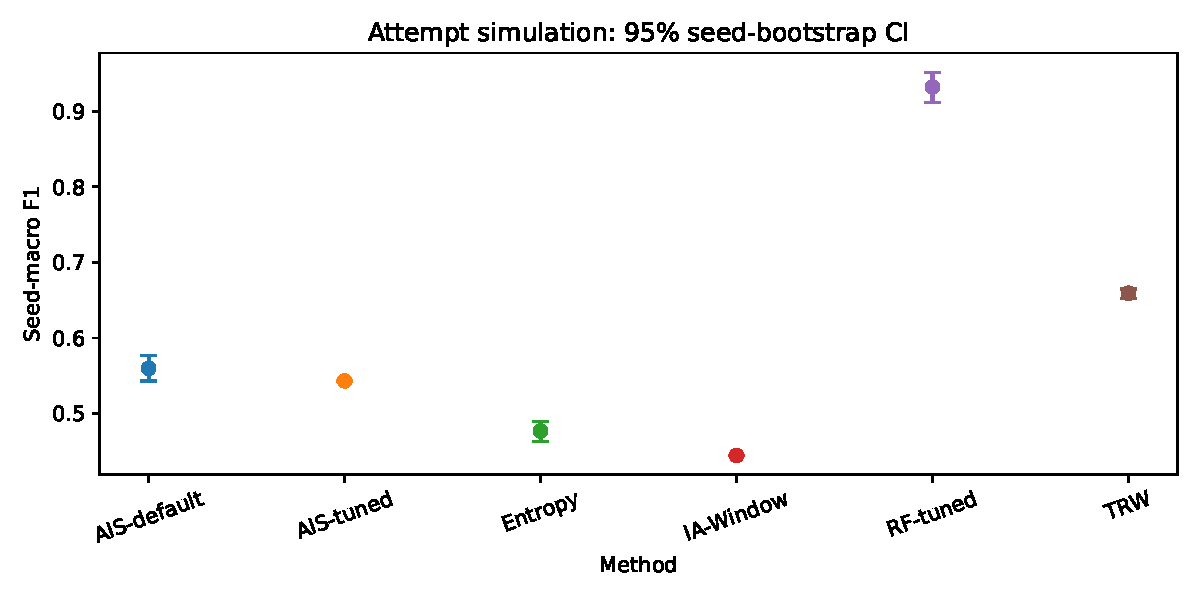
\includegraphics[width=.48\textwidth]{../results/research_simulation_v2/figures/01_F1_ci.pdf}
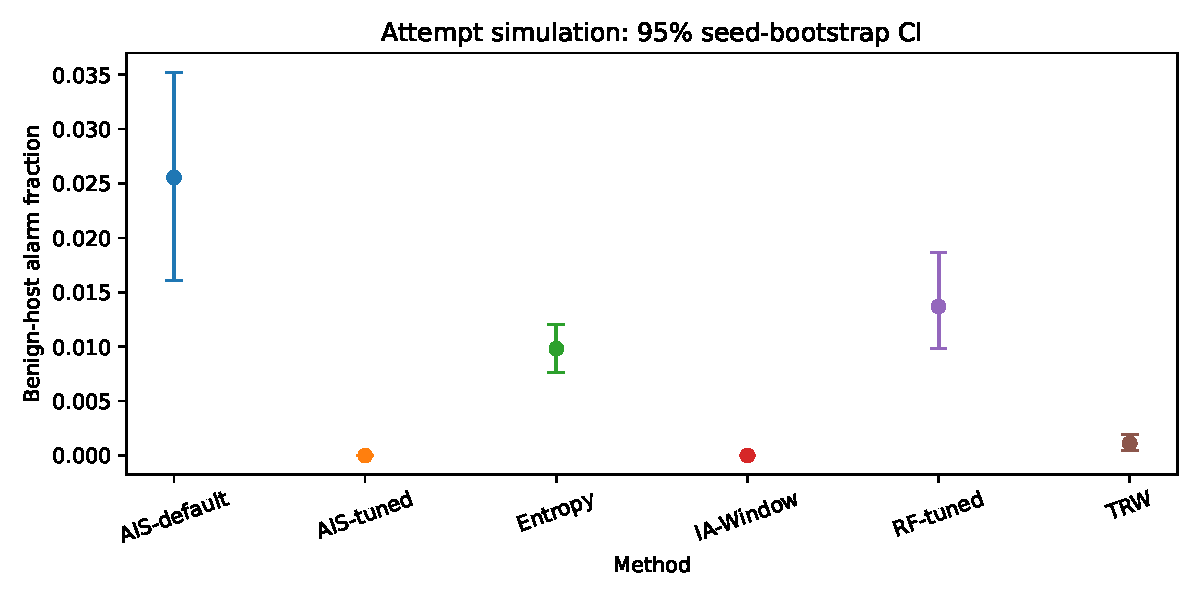
\includegraphics[width=.48\textwidth]{../results/research_simulation_v2/figures/02_FPR_ci.pdf}\\
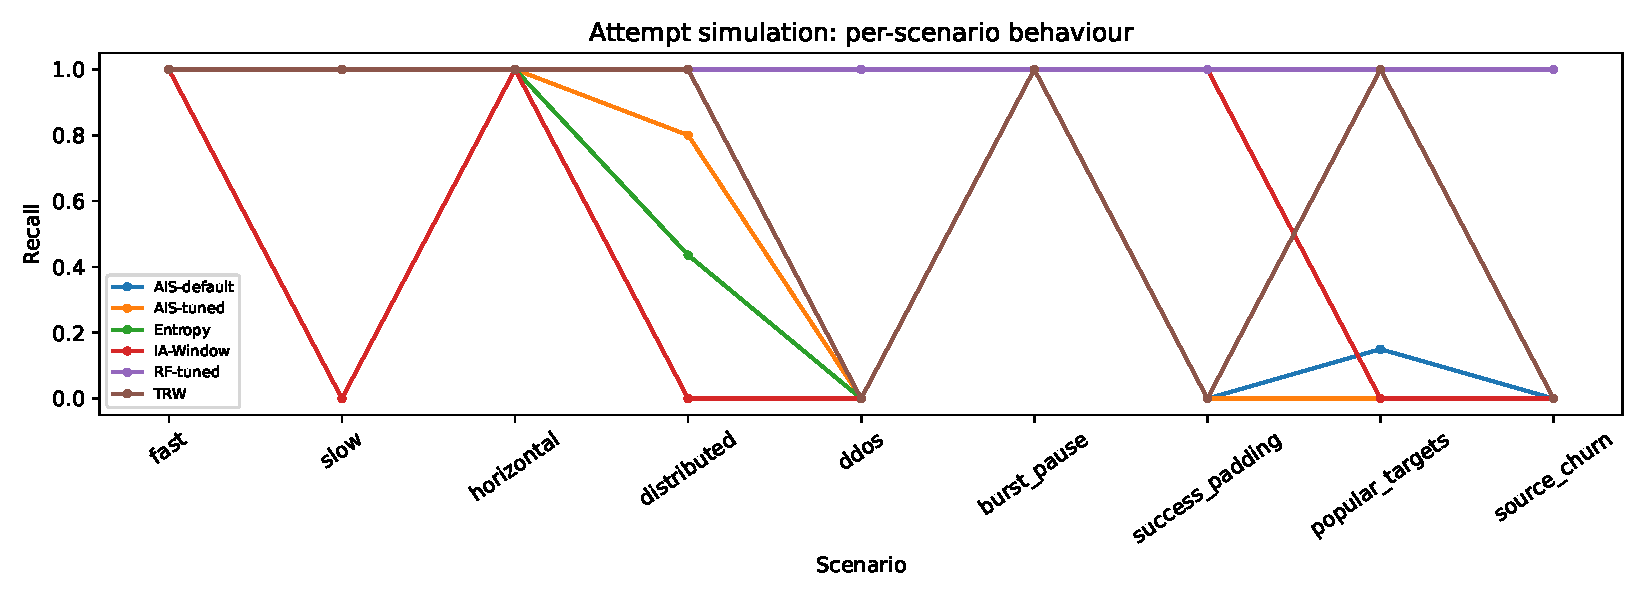
\includegraphics[width=.48\textwidth]{../results/research_simulation_v2/figures/03_scenario_TPR.pdf}
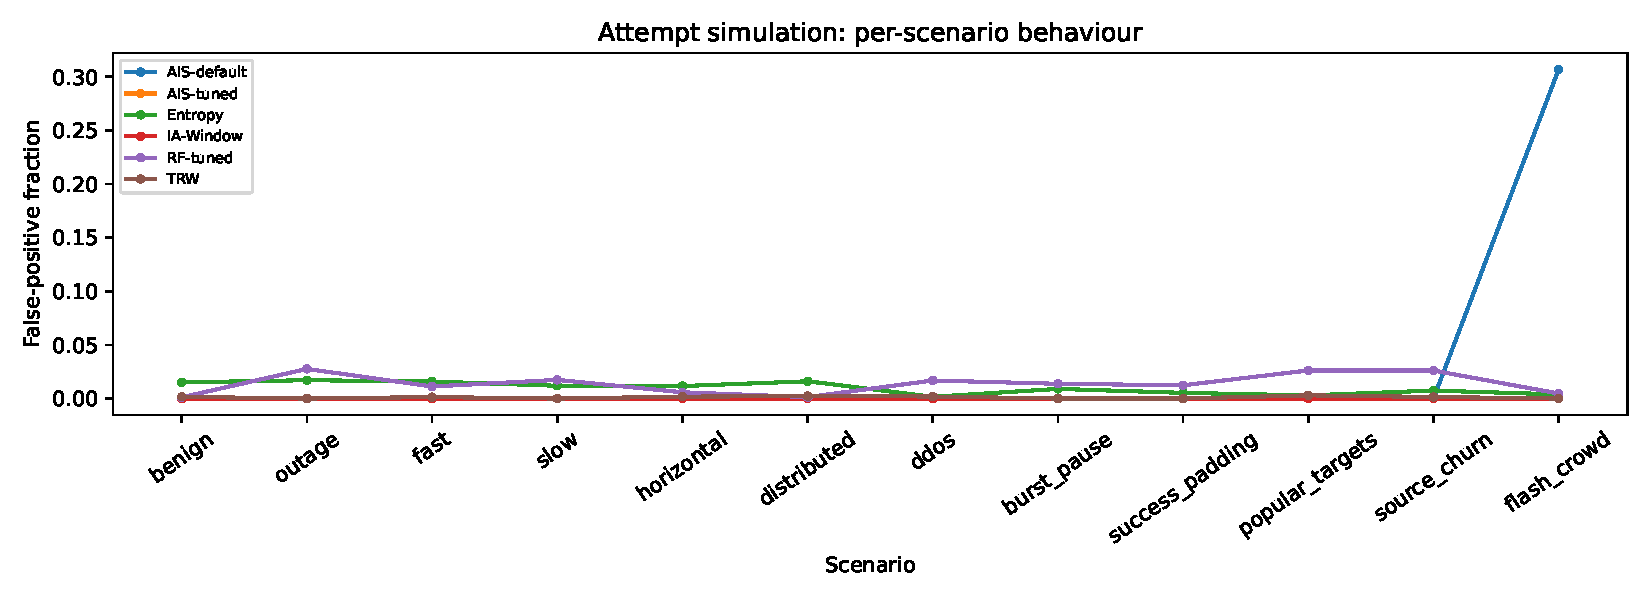
\includegraphics[width=.48\textwidth]{../results/research_simulation_v2/figures/04_scenario_FPR.pdf}
\caption{Additional attempt-level simulation: held-out F1/FPR uncertainty and scenario-level behaviour. F1 is macro
over attack scenarios within a seed; pure benign scenarios contribute to FPR. These are not new packet-capture results.}
\label{fig:extended-performance}
\end{figure*}

\subsection{Adaptive Strategies and Negative Results}
The twelve scenarios include burst/pause, success padding, probing popular targets, source churn, distributed scans,
low-per-source-rate distributed floods, outages and benign flash crowds. These are scripted adversarial strategies,
not a learned closed-loop attacker. Their strengths are varied on held-out seeds. A source-local detector can miss a
large distributed flood when each source remains below its rate allowance. Repeated popular targets suppress novelty
weights, while first-contact scoring limits the evidence available against a source that probes only a few services.
These cases must remain in the reported recall, rather than being excluded to preserve a perfect score.

\begin{figure*}[!tbp]
\centering
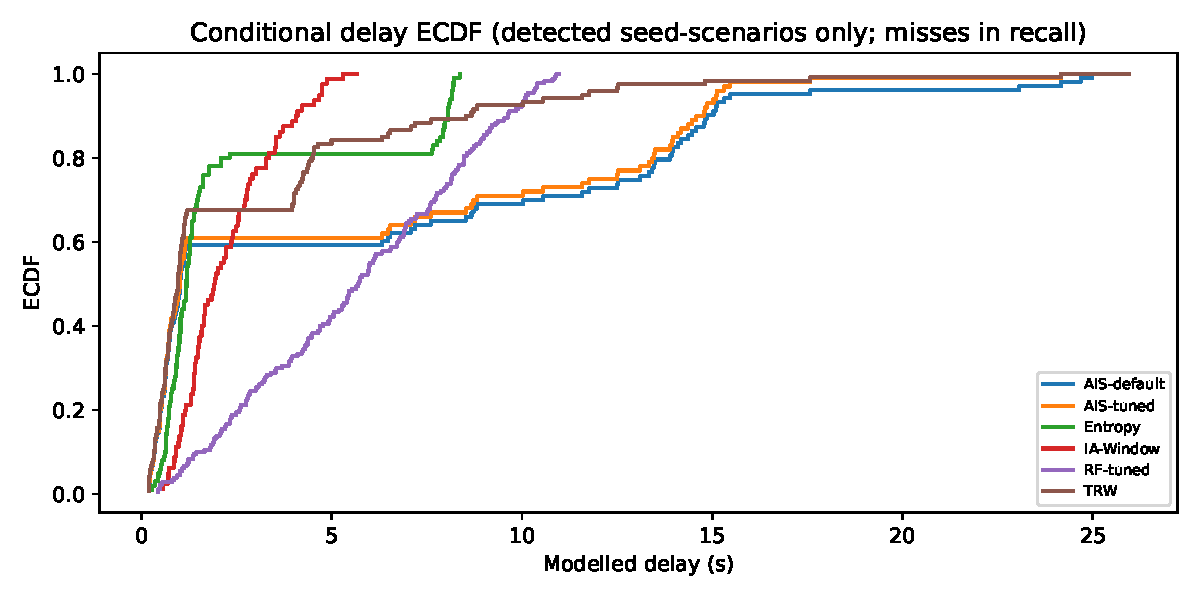
\includegraphics[width=.48\textwidth]{../results/research_simulation_v2/figures/05_delay.pdf}
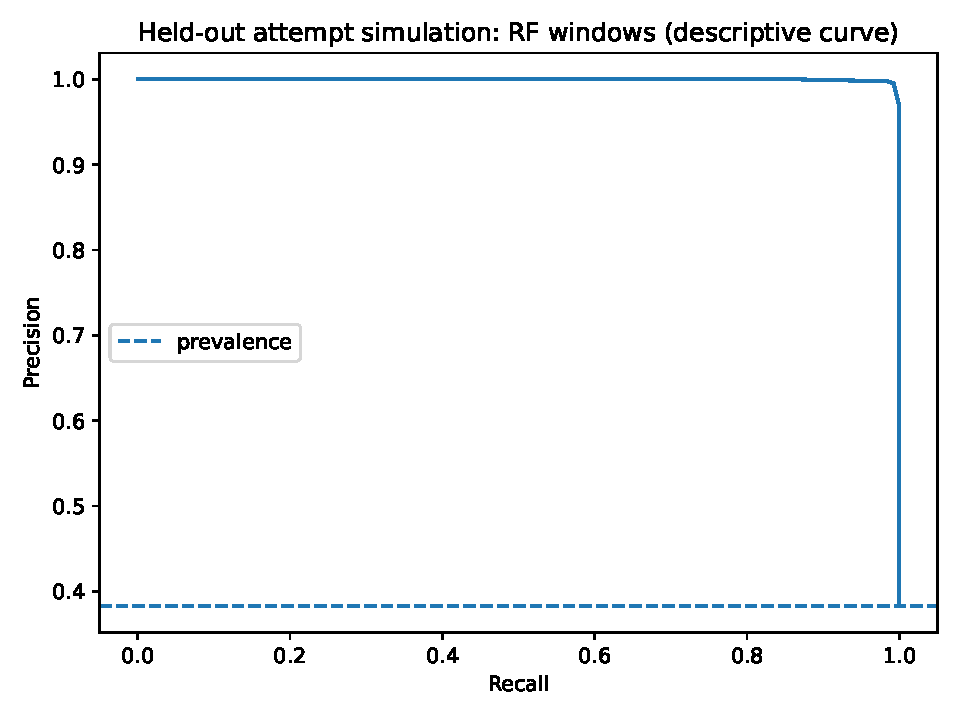
\includegraphics[width=.48\textwidth]{../results/research_simulation_v2/figures/06_RF_pr.pdf}\\
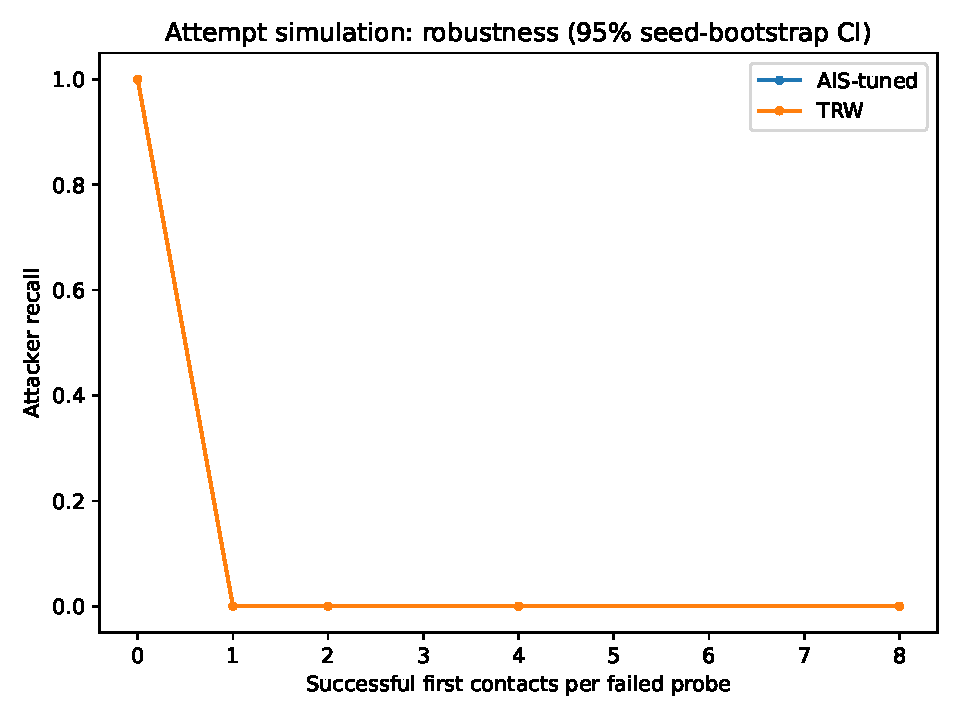
\includegraphics[width=.48\textwidth]{../results/research_simulation_v2/figures/07_padding.pdf}
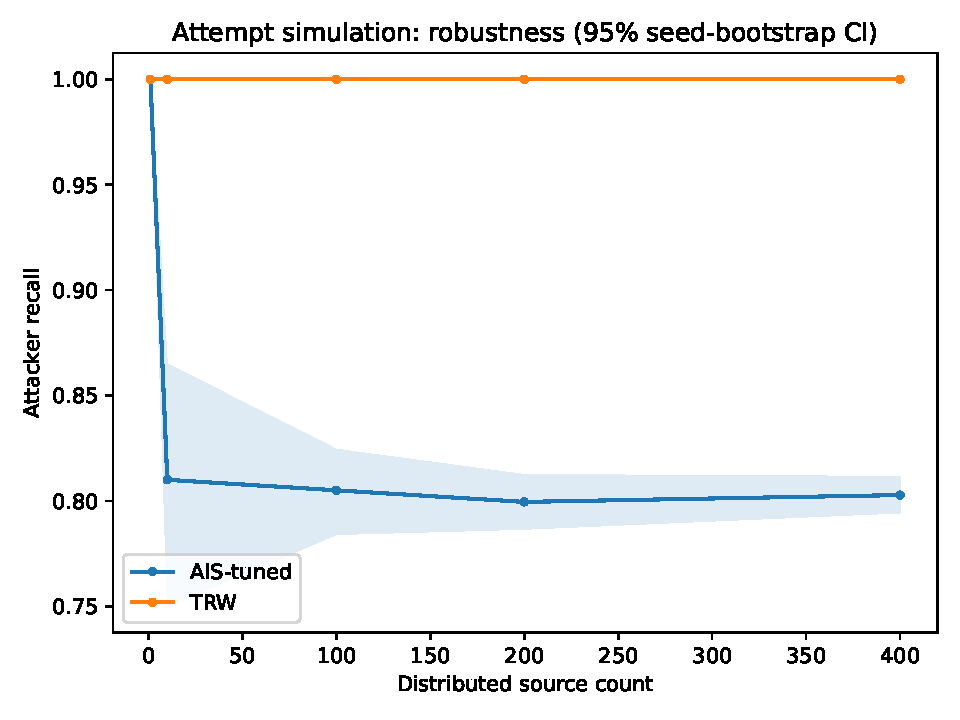
\includegraphics[width=.48\textwidth]{../results/research_simulation_v2/figures/08_sources.pdf}
\caption{Conditional detection-delay distribution, descriptive held-out RF precision--recall curve, success-padding
and distributed-source sensitivity. Missed detections are excluded from delay but retained in recall. The PR curve
does not select a new test-set operating threshold.}
\label{fig:extended-adaptive}
\end{figure*}

\subsection{Bounded State and Aging}
The revised streaming detector bounds active sources at 4,096 (3,600~s idle TTL), scored contacts at 65,536
(3,600~s since scoring), and services at 16,384 (3,600~s service-idle TTL). Capacity eviction is LRU. Each service
remembers at most 64 source identities; each source has at most 256 victim counters. The packet tracker bounds
pending resolutions at 65,536 and recently seen tuples at 131,072 (120~s idle TTL), instead of clearing its entire
seen set. Pending overflow is counted, not converted into fabricated failed connections. Cooldown keys are bounded
at 8,192. Periodic logs expose evictions, expiry and overflow.

The entry bound is $O(HV+C+SU+P+T+Q)$ for the stated host, victim, contact, service, service-user, pending,
tuple and cooldown limits; this is not a fixed RSS bound. Resource-pressure eviction can discard evidence and
reduce detection, so it is an explicit accuracy/resource trade-off. Offline PCAP extraction and materialized
evaluation events are not claimed to be bounded-memory streaming APIs.

\begin{figure*}[!tbp]
\centering
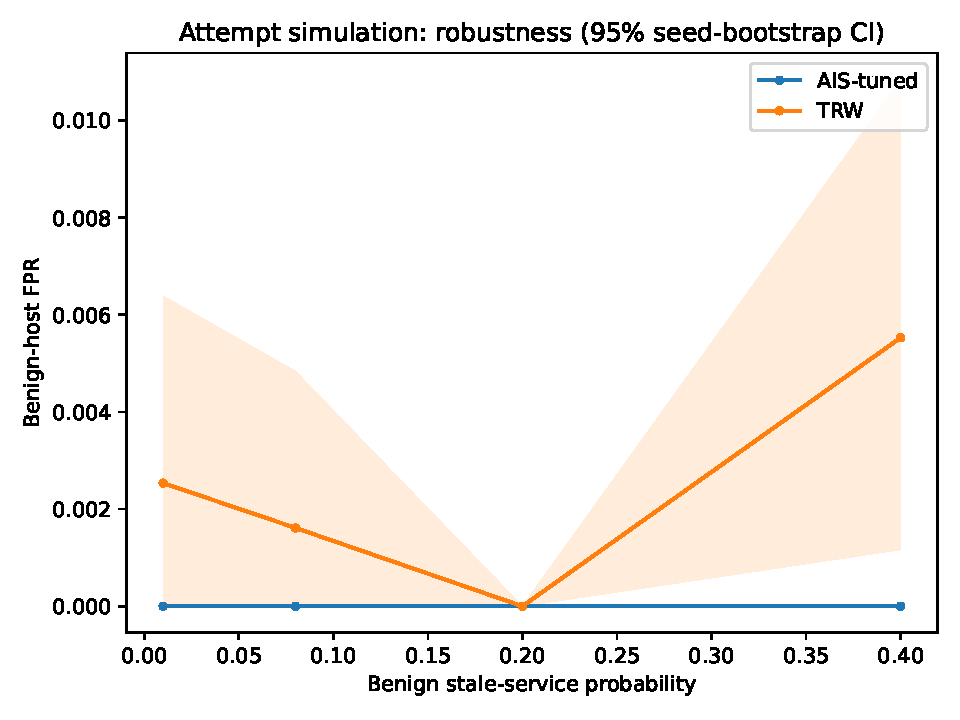
\includegraphics[width=.48\textwidth]{../results/research_simulation_v2/figures/09_failure.pdf}
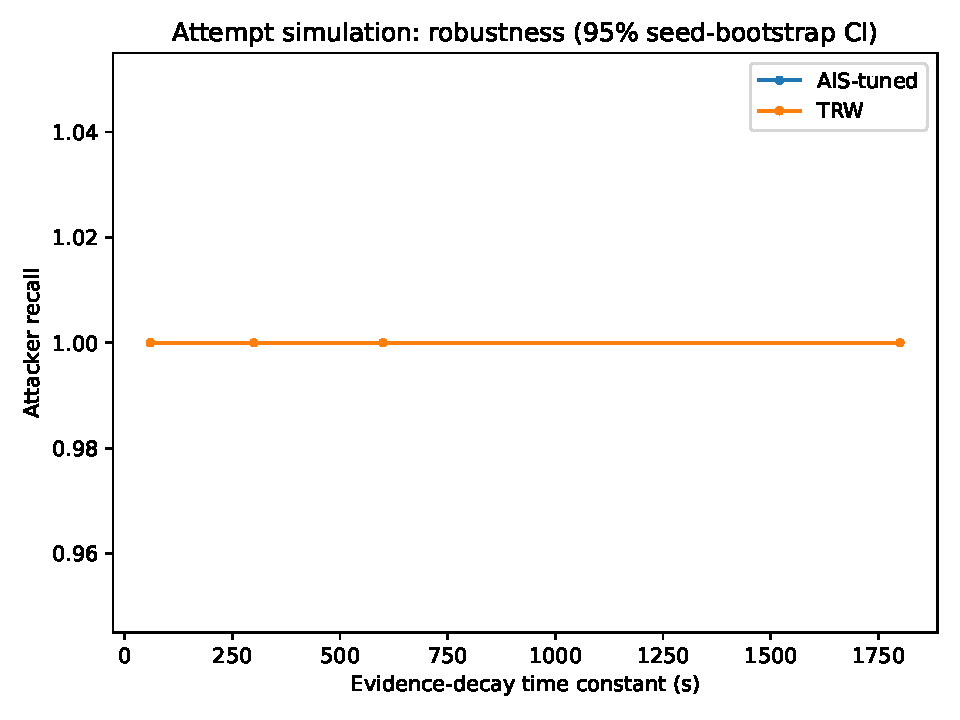
\includegraphics[width=.48\textwidth]{../results/research_simulation_v2/figures/10_tau.pdf}\\
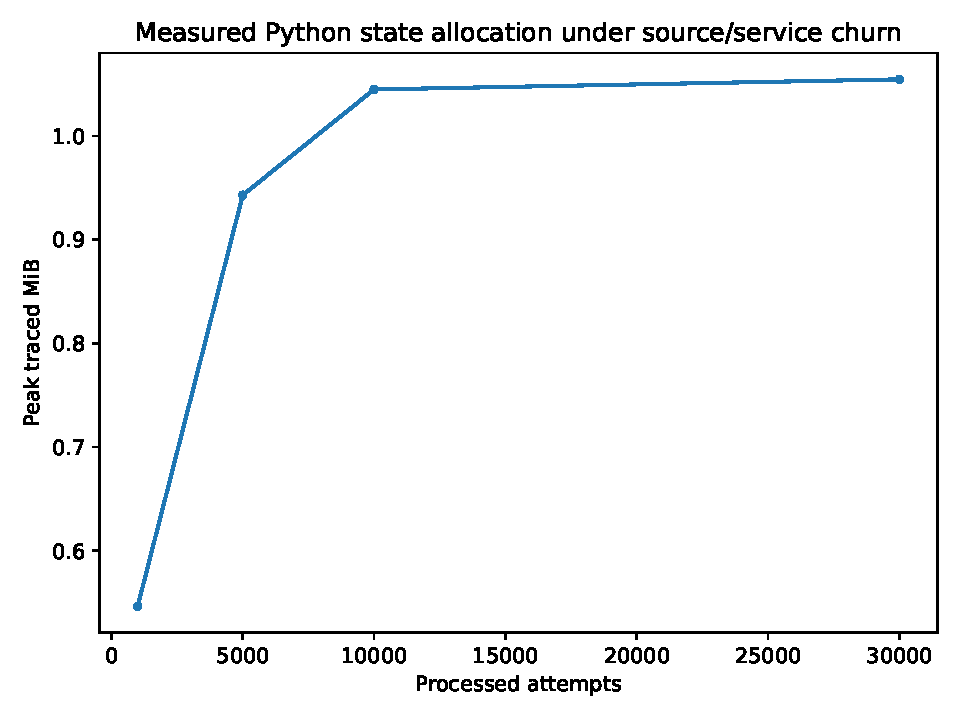
\includegraphics[width=.48\textwidth]{../results/research_simulation_v2/figures/13_memory.pdf}
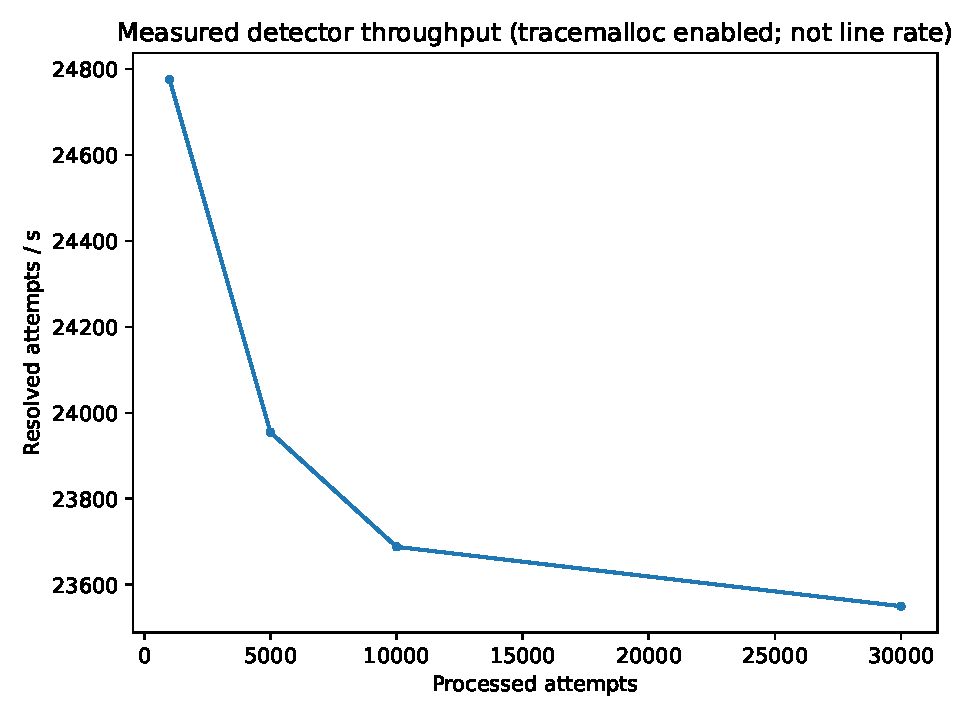
\includegraphics[width=.48\textwidth]{../results/research_simulation_v2/figures/14_throughput.pdf}
\caption{Benign-failure and decay sensitivity; measured traced Python memory and detector throughput under state
churn. The resource experiment uses smaller explicit caps ($H=256,C=2048,S=512$). Tracemalloc overhead is included;
throughput is resolved-attempt processing, not packet ingestion or switch line rate.}
\label{fig:extended-resources}
\end{figure*}

\subsection{Checking Proposition~\ref{prop:bounds}}
For each point we run 20,000 independent IID Bernoulli trials with the specified success probabilities and report exact
binomial 95\% intervals. The single-test recurrence stops at its first boundary. The restart recurrence instead resets
after each boundary over 400 observations. A third, finite-horizon toy recurrence uses 30~s gaps, $\tau=600$~s and
constant failure weight .5; it does not model service-popularity adaptation and does not establish a theorem.
Comparing the curves tests the assumptions of the proposition, not just classification accuracy.

\begin{figure*}[!tbp]
\centering
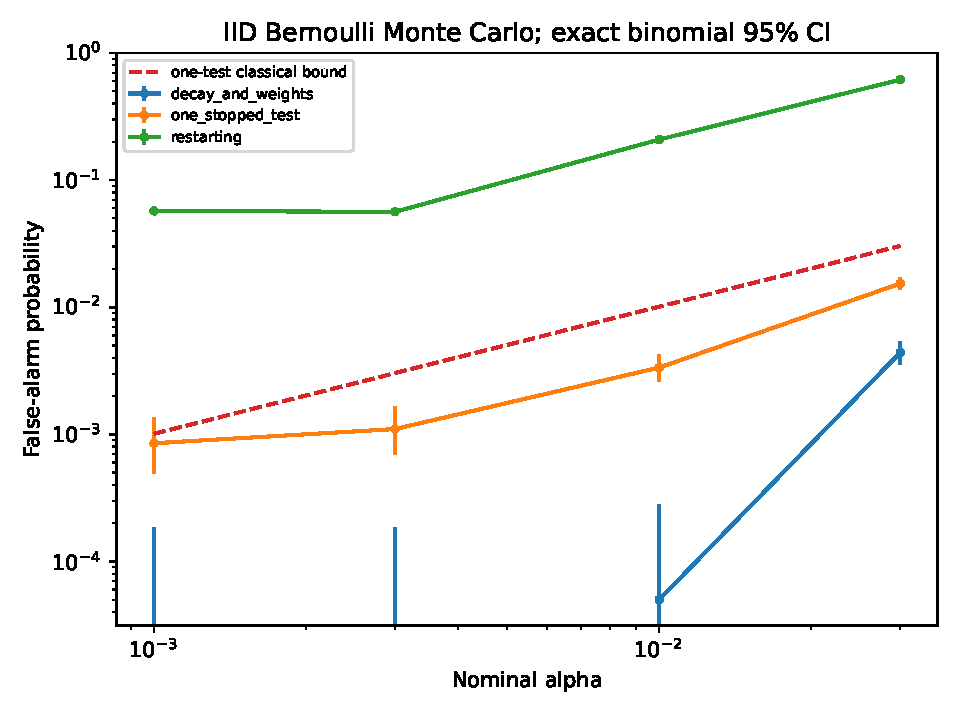
\includegraphics[width=.48\textwidth]{../results/research_simulation_v2/figures/11_bound_H0.pdf}
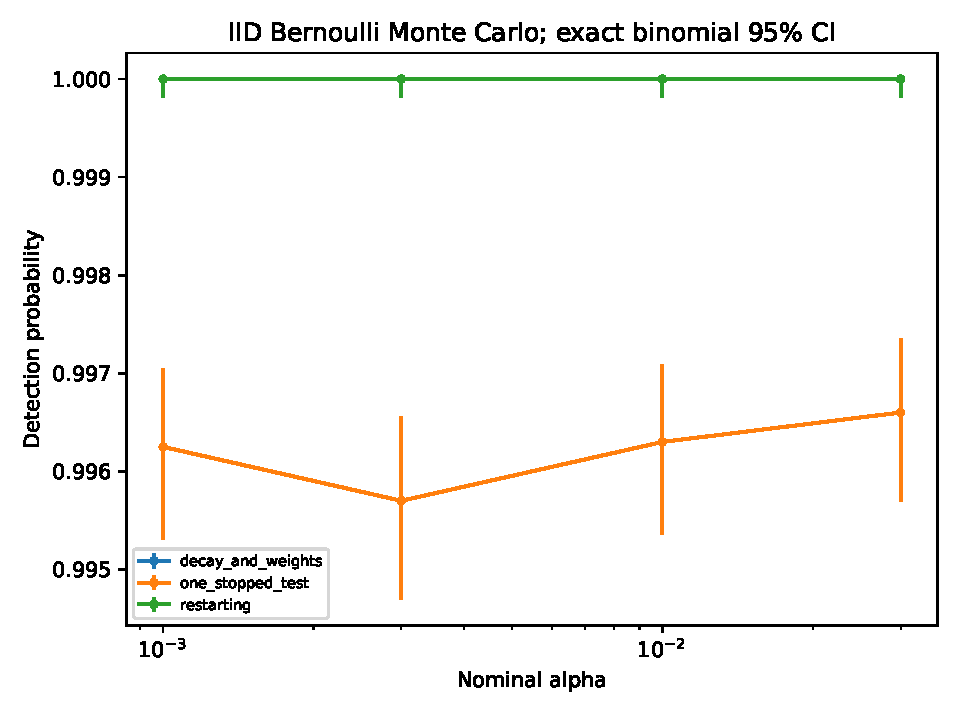
\includegraphics[width=.48\textwidth]{../results/research_simulation_v2/figures/12_bound_H1.pdf}
\caption{Empirical false-alarm and detection probabilities versus $\alpha$: one stopped classical test versus
restarting and a weighted/decayed finite-horizon recurrence. The classical false-alarm bound must not be attached
to the lifetime restarting detector.}
\label{fig:extended-bounds}
\end{figure*}

\subsection{Measured Enforcement and Remaining Network Evidence}
The separate WSL/Mininet experiment is a paired $2\times2$ design: fixed versus graded response and PacketIn guard
off versus on, with twenty held-out seeds and randomized arm order. It injects identical decisions to isolate
enforcement, not detection. Sender sequence IDs and receiver timestamps measure attacker packets arriving between
installation send and the final initial switch barrier ACK, collateral legitimate other-destination loss after an
injected false suspicion, installation delay and accepted repeat-offender block duration. Leakage includes packets
already in flight; it is not automatically evidence of the PacketIn race alone.
Only a complete 80-trial campaign may generate the paired-CI analysis. No missing measurement is replaced by simulation.
Large-source PCAP campaigns and RF evaluation use separate train/validation/test manifests; their completion status,
not the existence of a runnable script, determines which network-scale claims can be made.

% Generated from successful real-source smoke-trial metadata.
\newcommand{\ScaleSources}{200}
\newcommand{\ScalePackets}{159033}
\newcommand{\ScaleAttempts}{26485}

A separate 30~s DDoS smoke trial (seed 3001) validated \ScaleSources{} real attacking host namespaces plus twelve
benign hosts and two servers. The capture contains \ScalePackets{} packets and \ScaleAttempts{} resolved attempts,
with all requested source addresses observed after their individual onset times and zero reported kernel capture
drops. PCAP is spooled to native Linux storage before copying to the artifact; OVS port readiness and per-host
connectivity are checked before timed traffic. This is one validated scale trial, not twenty independent network
test seeds or evidence of high detection accuracy. The full 240-capture train/validation/test campaign was explicitly
deferred and remains future experimental work.

Finally, random synthetic traffic is not a substitute for multiple independently labelled public days/sites.
Success-conditioned trustworthy popularity, hierarchical evidence across low-rate sources, and anytime-valid
sequential error control are candidate research directions, not established novelty claims.
